\documentclass[a4paper,10pt]{article}

% Paquetes requeridos
\usepackage[utf8]{inputenc}
\usepackage[spanish]{babel}
\usepackage{csquotes}
\usepackage{amsmath, amssymb, amsfonts}
\usepackage{graphicx}
\usepackage[style=apa, backend=biber, natbib=true, language=spanish, url=true]{biblatex}
\usepackage{tocloft} % Para personalizar el índice
\usepackage[left=3.5cm,right=2.5cm,top=3.5cm,bottom=3.8cm]{geometry}
\usepackage{setspace} % Espaciado
\usepackage{titlesec} % Para personalizar los títulos
\usepackage{fancyhdr} % Para personalizar encabezados y pies de página
\usepackage{newtxtext}
\usepackage{ragged2e}

\pagestyle{fancy}
\fancyhf{} % Limpia encabezados y pies de página
\renewcommand{\headrulewidth}{0pt} % Elimina la línea del encabezado

\addbibresource{referencias.bib}
\DeclareLanguageMapping{spanish}{spanish-apa}
% Configuraciones
\setlength{\parskip}{6pt} % Espacio entre párrafos
\setstretch{1.15} % Espacio entre líneas

\renewcommand{\cftsecleader}{\cftdotfill{\cftdotsep}} % Para puntos en el índice

% Estilos para títulos y subtítulos
\titleformat{\section}
{\normalfont\fontsize{12}{15}\bfseries}{\thesection}{1em}{}
\titleformat{\subsection}
{\normalfont\fontsize{10}{13}\bfseries}{\thesubsection}{1em}{}
\titleformat{\subsubsection}
{\normalfont\fontsize{10.5}{13}\bfseries}{\thesubsubsection}{1em}{}

\usepackage[hypertexnames=false, colorlinks=true, 
linkcolor=blue, 
citecolor=blue, 
urlcolor=blue, 
linkbordercolor={1 1 0}, 
citebordercolor={1 1 0}, 
urlbordercolor={1 1 0}, 
filecolor=blue, 
pdfborderstyle={/S/U/W 1}]{hyperref}

% Inicio del documento
\begin{document}
	\pagestyle{empty}
	% Carátula
	\begin{titlepage}
		\centering
		\vspace*{1.5cm}
		{\fontsize{14}{17}\bfseries Scrum vs. Extreme Programming (XP): Una Comparativa y Orientación para la Elección de Metodologías Ágiles.\par}
		{\small Martin Borgo, Isaías Reniero, Leandro Molina\par}
		{\normalsize Universidad Nacional de Entre Ríos\par}
		{\normalsize Facultad de Ciencias de la Administración\par}
		{\normalsize Licenciatura en Sistemas\par}
		{\small \href{mailto:martinborgo8@gmail.com}{martinborgo8@gmail.com}, \href{mailto:isa.reniero001@hotmail.com}{isa.reniero001@hotmail.com}, \href{mailto:LeandroRodrigoMolina@gmail.com}{LeandroRodrigoMolina@gmail.com}\par}
		{\small \justify\textbf{Abstract.} Desde principios de los ‘90 comenzaron a surgir un amplia variedad de metodologías que se apartaban de los principios tradicionales de desarrollo de software. Estas nuevas metodologías sentaron las bases de lo que posteriormente se conocería como los valores ágiles, asentados unos años más tarde en el manifiesto ágil, de la mano de las figuras más importantes del mundo del desarrollo de software. En este artículo se comparará una de las metodologías más populares de principios de los años 2000 (eXtreme Programing) con una de las metodologías más utilizadas en la actualidad (Scrum), con el objetivo de ver sus diferencias y similitudes, ventajas y desventajas, estableciendo de forma clara las situaciones en las que se pueden aplicar cada uno de estos modelos.\par}
		
		{\small \textbf{Keywords:} Scrum, eXtreme Programming, Metodologías ágiles. \par}
	\end{titlepage}
	
	\section{Introducción}
	En el desarrollo de software, ágil (Agile) es una filosofía de desarrollo que incorpora una serie de prácticas, herramientas y una nueva cultura que permiten al equipo de desarrollo y a las partes interesadas colaborar estrechamente y prosperar en un entorno de requisitos en constante cambio, entregando un programa funcional de manera incremental e iterativa en periodos cortos de tiempo, obteniendo así una retroalimentación continua por parte del usuario. La filosofía ágil es intrínsecamente ligera y fomenta el trabajo en equipo, autoorganizados y empoderados para entregar software de alta calidad. En la actualidad existen distintas metodologías populares que siguen los valores y principios ágiles, tales como: XP \parencite{Beck_Andres_2005} Scrum \parencite{sutherland2014scrum}, Kanban \parencite{anderson2010kanban}, Lean \parencite{poppendieck2003lean}, Crystal \parencite{cockburn2004crystal}, DSDM \parencite{stapleton1997dynamic} y FDD \parencite{palmer2001practical}. Los valores son expresados y explicados en el manifiesto ágil \parencite{Manifesto_for_Agile_Software_Development}.
	
	Este artículo se centra en dos de las metodologías ágiles más prominentes: Scrum y eXtreme Programming (XP), ya que según estudios realizados por \textcite{fuior2019key} Scrum es una de las metodologías más utilizadas para el desarrollo de sistemas, mientras que XP es una de las menos utilizadas, este mismo resultado fue obtenido por el State of Ágil Report\footnote{\href{https://info.digital.ai/rs/981-LQX-968/images/SOA16.pdf}{16th State of Agile Report}} del 2022, donde XP ocupa una de las últimas posiciones, mientras que Scram se encuentra liderando la lista. Gracias a que estas metodologías gozan o han gozado de gran popularidad y se han sido utilizadas ampliamente en la industria del software como a nivel académico, proporcionando una abundante fuente de información, artículos científicos y casos prácticos. Este trabajo tiene como objetivo explorar las ventajas y desventajas individuales de cada metodología, proporcionando una visión de sus características distintivas y áreas de aplicación. Posteriormente, se revisarán diversas herramientas y estudios que han llevado a cabo comparando estas metodologías, con el objetivo de sintetizar los hallazgos y ofrecer una perspectiva equilibrada sobre cuándo es más apropiado utilizar una sobre la otra. Todo esto con la finalidad de brindar recomendaciones sólidas y basadas en evidencia para la selección de metodologías en situaciones específicas.
	\section{Desarrollo de Trabajo}
	En esta sección se realizará una breve introducción a cada una de las metodologías bajo estudio, describiendo tanto ventajas como desventajas, y se finalizará realizando una recopilación de estudios comparativos entre ambas metodologías, con el fin de comprobar los puntos expuestos y dar una visión más amplia sobre el tema.
	\subsection{eXtreme Programing}
	Desarrollado en 1999 por Kent Beck y Andres Cynthia, posteriormente presentado en su libro “\textit{Extreme Programming Explained: Embrace Change}” \parencite{Beck_Andres_2005}, XP es un marco de trabajo liviano orientado en su totalidad al desarrollo y entrega rápida de un producto de software, basada en un conjunto de buenas prácticas que debían ser llevadas a cabo para lograr los objetivos de manera correcta. Entre estas buenas prácticas se destaca la programación entre pares, la cual consiste en ubicar a dos programadores en un solo equipo, donde uno de ellos se encargará de escribir código y el otro observará dicho código corrigiendo posibles errores, estos roles se van rotando e incluso se puede ir alternando las parejas. Por otro lado está la refactorización, que a grandes rasgos consiste en hacer cambios en el código para hacerlo más legible, eficiente y mantenible, eliminando duplicaciones, mejorando la claridad del código y haciendo ajustes para seguir buenas prácticas de programación. Por último, se encuentra el desarrollo basado en pruebas o Test Driven Development \parencite{Beck_2003} por sus siglas en inglés, esta práctica se basa en un ciclo de desarrollo en el que se escribe una prueba, se escribe la cantidad mínima de código para que pase, se ejecutan todas las pruebas, para posteriormente refactorizar el código si es necesario. Este ciclo se repite hasta que todas las funcionalidades requeridas estén implementadas. Esta práctica, que en sus inicios fue propia de XP, resultó ser tan beneficiosa al momento del desarrollo que posteriormente fue implementada por otras metodologías de desarrollo como RUP, Kanban o incluso Scrum.
	
	Otra característica innovadora que propuso XP fue la idea de integrar al cliente o partes interesadas directamente en el proceso de desarrollo de software, esto con el fin de asegurar en primera instancia el verificar cumplimiento de los requerimientos del usuario o realizar los cambios que sean necesarios. Además este enfoque otorga ciertas ventajas a la hora de realizar correcciones en alguno de los requerimientos planteados, como también resulta más fácil el adaptarse a nuevos requerimientos que vayan surgiendo a lo largo del ciclo de vida del producto.
	
	\textcite{glass2001extreme} en su artículo menciona los aspectos positivos de XP, entre los cuales se encuentra el testeo unitario, que es probablemente una de las mejores prácticas en producción, la cual nos permite asegurar el buen funcionamiento de un componente del sistema, lo que evita futuros problemas en el desarrollo. Otro aspecto positivo destacado por el autor es la integración continua cuyo propósito es detectar los problemas que pueden surgir por la interacción entre las distintas partes que componen el sistema, garantizando de esta manera que el código escrito se puede combinar de manera efectiva. El último aspecto positivo que enfatizó Glass es el hecho de que el cliente está incluido desde el primer momento en el equipo de desarrollo y siempre es escuchado, presentando una ventaja por sobre Scrum, ya que solo el Product Owner es el único que interactúa con el cliente y la retroalimentación se produce recién en el Sprint Review, en cambio XP permite una retroalimentación más temprana y continua.
	
	Glass también destaca dos aspectos negativos presentes en XP. Por un lado nombra a la refactorización, si bien menciona que la práctica de este método es buena y permite mejorar el código escrito e incentiva a los programadores a utilizar estándares a la hora de codificar, esta práctica aplicada de forma incorrecta, muchas veces puede conducir al mal diseño de un componente o pieza del sistema, lo cual en proyectos medianos y grandes, esto se puede traducir en una gran cantidad de horas para reconstruir el componente por completo o en gran medida. El otro aspecto negativo que es mencionado en el artículo es la programación a pares. Este último aspecto  resulta ser sobre todo una opinión personal, ya que en un artículo publicado por \textcite{cockburn2000costs} demostró que si bien el tiempo de desarrollo de un equipo que emplea programación a pares es 15\% mayor en comparación con los grupos de desarrollo que programan de forma individual, la cantidad de errores en el código eran un 15\% menor en el caso de la programación a pares, esto representa un gran ahorro de tiempo y recursos, sobre todo de cara al mantenimiento. Además, los autores mencionan una gran cantidad de beneficios extras, tales como una mejora en la comunicación entre los miembros del equipo, una mejora significativa en cuanto al diseño del sistema y la mayor velocidad a la hora de resolver problemas, asimismo resulta útil de aplicar la programación a pares cuando en el grupo de trabajo existe personal que recién se incorpora al sector laboral, ya que estos pueden aprender mucho al programar de forma conjunta ya sea con personas más capacitadas o con el mismo nivel, gracias a la retroalimentación continua y mutua entre ambas partes.
	\subsection{Scrum}
	Scrum nace de un artículo publicado en el Harvard Business Review en 1986, titulado “\textit{El nuevo juego de desarrollo de nuevos productos}” \parencite{Takeuchi_Nonaka_1986}, en primera instancia este artículo estaba orientado al mundo industrial y no fue hasta que en 1993, Jeff Sutherland y su equipo en Easel Corporation tomaron y combinaron conceptos de ese artículo y crearon el proceso Scrum aplicado al desarrollo de software.
	
	Scrum se presenta como un marco de trabajo bien definido, más enfocado en la gestión del grupo de trabajo y el planeamiento de las diferentes tareas que se deben llevar a cabo en el proceso de desarrollo. El proceso de Scrum está compuesto por múltiples eventos (Sprint planning, Sprint review, Daily, Sprint retrospective), artefactos (Product Backlog, Sprint Backlog e Incremento) y roles (Product Owner, Scrum Master, Equipo de desarrollo) que son utilizados y llevados a cabo por distintas personas dentro del equipo de desarrollo. El aporte significativo de Scrum al campo de la ingeniería de software radica en su enfoque en la mejora continua del proceso de desarrollo. Al concluir cada iteración, o Sprint en el contexto de Scrum, se realiza un análisis del proceso de desarrollo llevado a cabo. Esto permite identificar áreas donde se puede mejorar y/o perfeccionar, dado que cada proyecto es único y puede requerir enfoques distintos para alcanzar el éxito y la correcta satisfacción del cliente.
	
	\textcite{rodriguez2015que} en su artículo dedican una sección a nombrar algunos aspectos en los que Scrum tiene algunas falencias con respecto a las demás metodologías ágiles que existen, entre esas falencias se encuentra el tiempo, el cual comparado con metodologías como XP donde el desarrollo y puesta en marcha del proyecto es mucho más veloz,  Scrum se encuentra en desventaja.  Por el lado de los requerimientos, la prioridad u orden en el que estos deben ser implementados dependen del Product Owner, lo cual implica que este puesto debe ser ocupado por una persona experimentada o con experiencia en la actividad. Por último se menciona como puede ser complicado adoptar Scrum en equipos de desarrollo con poca o nula experiencia en el desarrollo, ya que se requiere una sinergia muy grande entre el equipo de desarrollo, esto es respaldado por \textcite{barrios2012scrum} que en su artículo estudia cómo fue la aplicación de Scrum en una pequeña firma desarrolladora de software. El equipo de desarrollo estaba integrado en su mayoría por estudiantes universitarios con poca experiencia en el sector y por algunos graduados con experiencia previa en desarrollo, esto dio como resultado una mala coordinación inicial y estimación de los tiempos de desarrollo, aunque esto se fue corrigiendo en las siguientes Sprints, gracias a las Sprint retrospective. La estimación de los tiempos en Scrum también es una tarea difícil o cuanto menos complicada de realizar, ya que los plazos de tiempo estipulado para la implementación de una tarea es decidido arbitrariamente, ya sea por experiencias previas o suposiciones del equipo de desarrollo, lo que muchas veces se puede traducir en un incumplimiento de los plazos y por consiguiente una demora general en la planificación de las siguientes iteraciones.
	
	Una de las cosas positivas de Scrum es el hecho de que no define un proceso claro a la hora de su adopción, dejando esta decisión a manos del Scrum Master, esto brinda una gran flexibilidad, permitiendo adoptar tanto métodos como procesos de otras metodologías logrando adaptar mejor el desarrollo de acuerdo al tipo de sistema que se está construyendo, aunque este tipo de decisiones siempre deben tomarse con cautela. Una de las ventajas más destacadas de esta metodología es su capacidad de escalabilidad, como mencionamos al principio Scrum se enfoca en la gestión y organización de equipos de trabajo. Esto explica por qué empresas como Spotify eligen Scrum para el desarrollo de sus servicios. Sin embargo, es importante destacar que muchas empresas, incluyendo a Spotify, adaptan y personalizan la aplicación de Scrum para que se ajuste a sus necesidades específicas y al número de desarrolladores con los que cuentan \parencite{kniberg2012scaling}.
	\subsection{Estudios Comparativos}
	\textcite{Gill_Henderson-Sellers_2006} utilizaron una herramienta de análisis de 4 dimensiones (4-DAT) para evaluar y comparar las características de ambas metodologías. Esta herramienta permite analizar de manera formal las cualidades de cada una de las metodologías en base a 4 perspectivas llamadas dimensiones, las cuales son:
	\begin{enumerate}
		\item \textbf{Caracterización del alcance del método (Method Scope Characterization)}: Esta dimensión se enfoca en evaluar varios aspectos como el tamaño del proyecto, el estilo de desarrollo, el entorno tecnológico, etc., para determinar el alcance de un método ágil específico.
		\item \textbf{Caracterización de la agilidad (Agility Characterization)}: En esta dimensión, se evalúa el grado de agilidad de un método ágil en términos de características como flexibilidad, velocidad, leanness, aprendizaje y capacidad de respuesta. Es la única dimensión que tiene un enfoque cuantitativo dividida en dos (fases y prácticas).
		\item \textbf{Caracterización de los valores ágiles (Agile Values Characterization)}: Aquí se evalúa cómo un método ágil soporta los valores ágiles establecidos en el Manifiesto Ágil y otros identificados por los investigadores.
		\item \textbf{Caracterización del proceso de software (Software Process Characterization)}: Esta dimensión se centra en evaluar cómo un método ágil soporta diferentes procesos involucrados en el desarrollo de software, incluyendo el proceso de desarrollo, el proceso de gestión de proyectos, etc.
	\end{enumerate}
	Tres de estas dimensiones son cualitativas, solamente una (Agility Characterization) es cuantitativa. Se usan estas dimensiones para analizar y comparar las metodologías a través de tablas\footnote{Los autores además comentan que han desarrollado un prototipo para la implementación de medición de agilidad (Gill \& Henderson-Sellers, 2006, p. 1)}, ya que cada dimensión contiene diferentes aspectos de estas.
	
	La primera dimensión se utiliza para analizar y comparar el alcance de XP y Scrum en varios aspectos como el tamaño del proyecto, el tamaño del equipo, el estilo de desarrollo, entre otros. Se encuentran que ambos métodos son adecuados para proyectos pequeños y medianos, pero Scrum puede escalar para proyectos grandes, este mismo resultado fue obtenido por \textcite{quinonez2017analisis} en su artículo donde se comparaban las distintas metodologías ágiles.
	
	La segunda dimensión mide el grado de agilidad en términos de flexibilidad, velocidad, leanness\footnote{En el contexto de los métodos ágiles se refiere a la eficiencia y economía del proceso de desarrollo. Un proceso "lean" (delgado, en español) busca eliminar el desperdicio, es decir, cualquier cosa que no agregue valor al producto final, y se enfoca en proporcionar exactamente lo que el cliente necesita, ni más ni menos.}, aprendizaje y capacidad de respuesta, asignando una calificación de 1 o 0, donde 1 es positivo y 0 es negativo. Este análisis se realiza en dos niveles: fases y prácticas. Las "fases" se refieren a las etapas del ciclo de vida del desarrollo del software. Y las "prácticas" se refiere a las técnicas específicas empleadas dentro de cada método, como "The Planning Game" en XP, o "Product Backlog" en Scrum. A partir de este análisis, se pueden sacar las siguientes conclusiones:
	% poner imagen
	La tercera dimensión analiza cómo las prácticas de XP y Scrum representan los valores ágiles del Manifiesto Ágil. Ambas metodologías respaldan firmemente los primeros cuatro valores a través de varias prácticas. No obstante, XP no respalda los valores de "mantener el proceso ágil" y "mantener el proceso rentable". Scrum respalda el primero, pero, igual que XP, no sostiene el compromiso con la rentabilidad del proceso.
	
	La cuarta dimensión examina las prácticas de XP y Scrum para el desarrollo y gestión de proyectos de software. Ambas metodologías presentan prácticas sólidas para estos aspectos, pero no abordan directamente el "Proceso de Control de Configuración/Soporte" ni el "Proceso de Gestión del Proceso". XP destaca por su amplia gama de prácticas que respaldan el desarrollo. Scrum, en cambio, pone un mayor énfasis en el trabajo en equipo y las iteraciones regulares para impulsar el desarrollo. Ambos ofrecen enfoques distintos pero efectivos para la gestión de proyectos.
	
	Si bien esta herramienta resulta útil para la toma de decisiones tiene una serie de limitaciones. Primero, la asignación binaria (0 o 1) para cada característica puede ser demasiado simplista, no capturan la variabilidad y complejidad de cada fase y práctica. Segundo, el análisis es en gran parte cualitativo, lo que puede introducir subjetividad y limitar la precisión del análisis. Tercero, la cantidad de prácticas evaluadas en cada metodología puede influir en los resultados, potencialmente favoreciendo a la metodología con menos prácticas.
	
	Por otro lado, \textcite{fernandes2010classification} realizan una comparación de XP y Scrum en base a un modelo propuesto por \textcite{sol1983feature} en donde se realiza un análisis cuasi formal de cada una de las metodologías en base a su propuesta y su aplicación práctica. El análisis se divide en dos partes, la primera evalúa cómo se satisface los requerimientos de software en base a 5 atributos. La segunda parte se centra en los aspectos relacionados a la construcción de software, que a su vez es evaluado en base a 4 atributos. A cada uno de estos atributos se le asigna una nota conceptual (satisfecho adecuadamente, parcialmente satisfecho y no satisfecho) basándose en la teoría existente sobre la metodología y su implementación en casos prácticos. Lo más interesante del análisis realizado por Fernandez y Almeida es que dado que Scrum fue planteado desde un inicio como un marco de trabajo orientado a la organización de las distintas tareas y actividades, en el apartado de construcción de software concretamente en todos sus sub-atributos fueron puestos como no satisfechos, aunque en la síntesis de los resultados se lleva un gran puntaje en el apartado de gestión.
	
	Otros autores optan por un enfoque distinto a la hora de la selección de una de estas metodologías. \textcite{perez2012guia} enfatiza que para la elección e implementación de una metodología, previamente debe haber una exhaustiva documentación, comprendiendo el marco de la organización, es por eso que el autor propone una serie de cuestionarios. Los datos recopilados de estos formularios se comparan con las clasificaciones de las metodologías, que el autor presenta en una tabla. Al comparar los resultados del formulario con la tabla de clasificación de metodologías, se identifica cuál de ellas se adapta mejor al enfoque de trabajo de la organización. Dicha tabla nos permite observar que XP obtiene el puntaje más alto cuando la organización se centra en el desarrollo de software. Mientras que Scrum obtiene el puntaje más alto cuando la organización se centra mayormente en la gestión de proyectos y la exhaustiva estructuración de los tiempos.
	
	\section{Resultados Obtenidos}
	La tabla \ref{tabla_ventajas_desventajas} presenta en forma de resumen, a grandes rasgos, las ventajas y desventajas de XP y Scrum discutidas en las subsecciones anteriores.
	\begin{figure}[h]
		\centering
		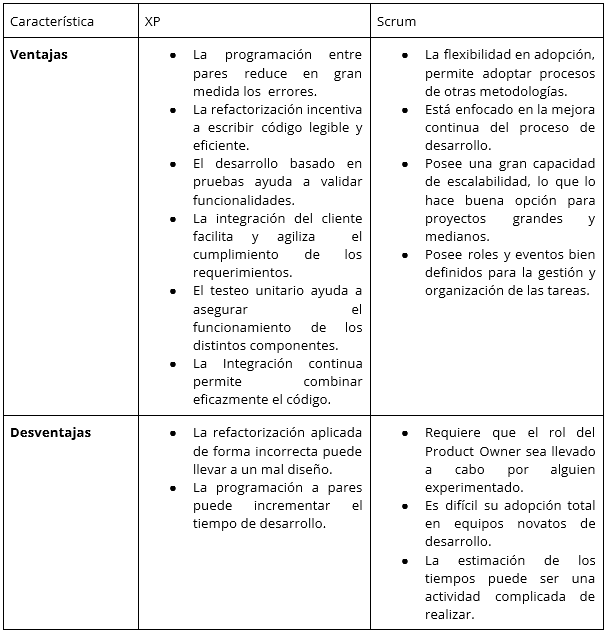
\includegraphics[width=0.7\textwidth]{tablaVentajasDesventajas.PNG}
		\caption{Tabla ventajas y desventajas de XP/Scrum}
		\label{tabla_ventajas_desventajas}
	\end{figure}\newline
	Por el lado de los estudios comparativos, en términos generales Scrum resulta una opción mucho más preferible a la hora de la gestión de un sistema de software ya que la flexibilidad y escalabilidad son factores mucho más preferibles a la hora de llevar adelante un proyecto. XP, no se caracteriza por su proceso, sino por el conjunto de estrategias y prácticas que aplicadas de la forma correcta aumentan enormemente la calidad de un producto de software. Con la ventaja de que estas mismas pueden ser, de hecho, son aplicadas por múltiples metodologías, por ejemplo aplicar TDD durante el desarrollo de un Sprint de Scrum.

	\section{Conclusión}
	Este artículo expuso las ventajas y desventajas de cada una de estas metodologías, además de realizar una recopilación de estudios comparativos entre estas mismas, donde se corroboró que a la hora de seleccionar uno de estos enfoques se debe considerar el tamaño del equipo de desarrollo, el tamaño de la empresa, la naturaleza del proyecto, la cultura organizacional, el nivel de conocimiento del personal involucrado, entre otros aspectos. Si bien cada modelo es aplicable ante distintas situaciones, no es necesario restringirse y enfocarse solamente en una única metodología por sobre la otra. Ya que como plantea \textcite{bahit2012scrum} gracias a que ninguno de estos marcos de trabajos son restrictivos, es posible adoptar y combinar las distintas prácticas presentes en estos modelos de la forma que resulten más convenientes para el proyecto, esta práctica es algo recurrente en la industria, lo que genera como resultado la implementación de forma híbrida de varias metodologías, entre ellas XP/Scrum o Scrum/XP. Las cuales ofrecen todas las ventajas de ambas metodologías e incluso resuelven algunas de las falencias presentes en el framework original.
	
	\nocite{*}
	\printbibliography[heading=bibintoc]
\end{document}
